\documentclass[UTF8,a4paper,12pt]{ctexart}

% ==================== 宏包 ====================
\usepackage{geometry}
\geometry{top=2.5cm,bottom=2.5cm,left=2.5cm,right=2.5cm}
\usepackage{amsmath,amssymb,bm}
\usepackage{booktabs,tabularx,array,multirow,longtable}
\usepackage{graphicx}
\usepackage{float}
\usepackage{placeins}
\usepackage{caption}
\usepackage{enumitem}
\usepackage{titlesec}
\usepackage{xcolor}
\usepackage{listings}
\usepackage{fvextra}
\usepackage{multicol}
\usepackage{xurl}
\usepackage{gbt7714}
\usepackage{hyperref}
\hypersetup{hidelinks}
\usepackage{fancyhdr}

% ==================== 基本版式 ====================
\setlength{\parindent}{2em}
\setlength{\parskip}{0pt}
\linespread{1.25}
\captionsetup{font=small,labelsep=quad}
\numberwithin{equation}{section}

% 正文页右上角队伍控制号
\newcommand{\TeamControlNumber}{TJMML2026393}
\pagestyle{fancy}
\fancyhf{}
\setlength{\headheight}{14pt}
\fancyhead[R]{\small 队伍控制号：\TeamControlNumber}
\fancyfoot[C]{\thepage}
\renewcommand{\headrulewidth}{0pt}

\floatname{algorithm}{算法}


% ---------- 只需修改的基本信息 ----------
\newcommand{\PaperTitle}{低空经济背景下的多无人机协同巡检路径优化}

% ---------- 正文版式 ----------
\setlength{\parindent}{2em}
\setlength{\parskip}{0pt}
\linespread{1.30}
\setlength{\abovedisplayskip}{8pt plus 2pt minus 2pt}
\setlength{\belowdisplayskip}{8pt plus 2pt minus 2pt}

\captionsetup{font=small,labelsep=quad}
\renewcommand{\figurename}{图}
\renewcommand{\tablename}{表}
\renewcommand{\refname}{参考文献}

% 一级标题用“一、二、三”，二级及以下用“1.1、1.1.1”。
\renewcommand{\thesection}{\chineseSection{section}}
\newcommand{\chineseSection}[1]{%
  \ifcase\value{#1}\or 一\or 二\or 三\or 四\or 五\or 六\or 七\or 八\or 九\or 十\or 十一\or 十二\else\arabic{#1}\fi}
\renewcommand{\thesubsection}{\arabic{section}.\arabic{subsection}}
\renewcommand{\thesubsubsection}{\arabic{section}.\arabic{subsection}.\arabic{subsubsection}}


% ---------- 页眉页脚 ----------
% 摘要页和目录页：只显示页脚居中页码。
\fancypagestyle{frontmatter}{
  \fancyhf{}
  \fancyfoot[C]{\thepage}
  \renewcommand{\headrulewidth}{0pt}
  \renewcommand{\footrulewidth}{0pt}
}
% 正文、参考文献、AI 使用说明和附录：右上角显示队伍控制号。
\fancypagestyle{mainmatter}{
  \fancyhf{}
  \fancyhead[R]{\small 队伍控制号：\TeamControlNumber}
  \fancyfoot[C]{\thepage}
  \renewcommand{\headrulewidth}{0pt}
  \renewcommand{\footrulewidth}{0pt}
}

% ---------- 公式、代码和占位内容 ----------
\numberwithin{equation}{section}

\lstdefinestyle{paperstyle}{
  basicstyle=\ttfamily\small,
  numbers=left,
  numberstyle=\tiny\color{gray},
  frame=single,
  breaklines=true,
  showstringspaces=false,
  columns=fullflexible,
  keywordstyle=\color{blue!65!black},
  commentstyle=\color{green!40!black},
  stringstyle=\color{orange!60!black}
}
\lstset{style=paperstyle}

% 附录中的源程序采用可断行的双栏逐文件排版。
\newcommand{\CodeFile}[2]{%
  \par\medskip
  \noindent\textbf{#1}\par
  \noindent\textbf{路径：}\nolinkurl{#2}\par\smallskip
  \VerbatimInput[
    fontsize=\tiny,
    numbers=left,
    numbersep=3pt,
    frame=lines,
    framesep=1mm,
    rulecolor=\color{black!30},
    breaklines=true,
    breakanywhere=true,
    tabsize=4
  ]{#2}
}

\begin{document}
\pagenumbering{arabic}
\setcounter{page}{1}

% =============================================================
% 第 1 页：摘要页（不得出现姓名、学院等身份信息；不得超过一页）
% =============================================================
\pagestyle{frontmatter}
\thispagestyle{frontmatter}

\begin{center}
  \vspace*{0.7cm}
  {\bfseries\fontsize{20pt}{28pt}\selectfont \PaperTitle\par}
  \vspace{0.9cm}
  {\bfseries\fontsize{16pt}{22pt}\selectfont 摘\quad 要\par}
\end{center}

\vspace{0.35cm}

针对不同等级巡检点需要重复访问、同一架无人机不能通过原地停留重复计数以及临时管制区随时间生效的多无人机协同巡检问题，本文将每次有效巡检转化为独立任务副本，建立由机队规模、系统完成时间和单机工时均衡性构成的递进式路径优化模型。

对于问题一，将任务建模为带重复巡检与最大工时约束的 Min--Max 多旅行商问题，利用总服务时间和最小生成树构造机队规模下界，再结合加权 K-means、极角扫描、合法插入、2-opt 与模拟退火搜索闭合路线。四个算例当前采用的无人机数量分别为 $4,2,5,4$ 架，对应最长工作时间分别为 $8.6111,7.5890,8.2876,8.6263$ h，均满足9小时限制。其中 Case 2 和 Case 4 的可行数量与理论下界相等，机队规模达到理论最小值；Case 1 和 Case 3 的结果为当前已验证的最小可行候选。

对于问题二，固定问题一采用的机队规模，并约束总体完成时间不劣于问题一方案，通过重载路线任务迁移、跨路线交换和 2-opt 重新分配实际工作量。四个算例的单机工时极差分别降至 $0.0174,0.0103,0.0238,0.0077$ h，较问题一分别下降 $72.1\%,9.7\%,41.8\%,62.6\%$，且未通过额外等待制造表面均衡。

对于问题三，以8:00为时间原点，在固定机队规模下建立圆形管制区的时空联合约束，构造时变可见图，同时比较安全等待与空间绕飞，并采用 $\varepsilon$-约束两阶段算法依次优化总体完成时间和工时极差。四个算例所得最长工作时间分别为 $8.6111,13.1404,9.6280,10.9250$ h；其中 Case 2 的必要等待由基准算法的 $189.297$ min 降至 $47.645$ min。全部正式方案及机队规模敏感性结果均通过独立逐事件复核。本文所得数值为给定计算预算内的最好可行结果，不将启发式搜索结果表述为已经证明的全局最优解。

\vspace{0.45cm}
\noindent\textbf{关键词：}多无人机协同巡检；Min--Max 多旅行商问题；负载均衡；时变可见图；词典序优化
\vspace{0.45cm}

% =============================================================
% 第 2 页：目录页
% =============================================================
\clearpage
\pagestyle{frontmatter}
\thispagestyle{frontmatter}

\begin{center}
  \vspace*{0.35cm}
  {\bfseries\fontsize{18pt}{24pt}\selectfont 目\quad 录\par}
\end{center}
\vspace{0.45cm}

% 本页按定稿的实际页码手工编排，不读取 .toc 文件。
\newcommand{\TOCSection}[3]{%
  \noindent\makebox[2.3em][l]{\bfseries #1、}%
  \textbf{#2}\dotfill\textbf{#3}\par}
\newcommand{\TOCSubsection}[3]{%
  \noindent\hspace*{2.3em}\makebox[2.8em][l]{#1}#2\dotfill#3\par}
\begingroup
  \setlength{\parskip}{0.08em}
  \linespread{1.02}\selectfont
  \TOCSection{一}{问题重述}{3}
  \TOCSubsection{1.1}{问题背景}{3}
  \TOCSubsection{1.2}{问题要求}{3}
  \TOCSection{二}{问题分析}{3}
  \TOCSubsection{2.1}{问题一分析}{3}
  \TOCSubsection{2.2}{问题二分析}{4}
  \TOCSubsection{2.3}{问题三分析}{4}
  \TOCSection{三}{模型假设}{4}
  \TOCSection{四}{主要符号说明}{5}
  \TOCSection{五}{问题一的模型建立与求解}{5}
  \TOCSubsection{5.1}{模型建立}{5}
  \TOCSubsection{5.2}{求解方法}{8}
  \TOCSubsection{5.3}{计算结果与分析}{10}
  \TOCSection{六}{问题二的模型建立与求解}{11}
  \TOCSubsection{6.1}{递进模型与均衡目标}{11}
  \TOCSubsection{6.2}{均衡优化算法}{12}
  \TOCSubsection{6.3}{计算结果与分析}{12}
  \TOCSection{七}{问题三的模型建立与求解}{14}
  \TOCSubsection{7.1}{动态管制模型}{14}
  \TOCSubsection{7.2}{求解方法}{15}
  \TOCSubsection{7.3}{计算结果与分析}{17}
  \TOCSection{八}{模型检验与敏感性分析}{19}
  \TOCSubsection{8.1}{问题一、问题二结果复核}{19}
  \TOCSubsection{8.2}{问题三独立可行性检验}{20}
  \TOCSubsection{8.3}{问题三机队规模敏感性分析}{20}
  \TOCSection{九}{模型评价与推广}{21}
  \TOCSubsection{9.1}{模型优点}{21}
  \TOCSubsection{9.2}{模型不足与改进}{21}
  \noindent\textbf{参考文献}\dotfill\textbf{23}\par
  \noindent\textbf{人工智能工具使用说明}\dotfill\textbf{25}\par
  \noindent\textbf{附录}\dotfill\textbf{26}\par
\endgroup

% =============================================================
% 第 3 页起：正文；从本页开始右上角显示队伍控制号
% =============================================================
\clearpage
\pagestyle{mainmatter}
\thispagestyle{mainmatter}

\section{问题重述}
\subsection{问题背景}
低空经济的发展使无人机逐渐应用于分散设施和低空航路的日常巡检。与单次访问问题不同，本题的巡检点具有不同等级，对应不同的重复巡检次数；无人机必须从同一基地出发并返回，且同一架无人机不能通过在原地连续停留重复计数。实际执行中还会出现带有生效时段的临时圆形飞行管制区，使路线可行性同时受到空间位置和通过时刻的影响。因此，需要在有限工作时间和动态管制条件下，统筹机队规模、任务分配、访问顺序与工作负载均衡。

\subsection{问题要求}
问题一根据附件一给出的四组巡检点坐标和等级，在9小时内完成全部有效巡检并返回基地，确定各算例采用的无人机数量和协同路线，使机队规模及系统总体完成时间尽可能小。问题二固定问题一采用的机队规模，在不恶化总体完成时间的条件下重新分配任务和调整访问顺序，缩小无人机之间的工作时间极差。问题三进一步结合附件二给出的圆形管制区及生效时间窗，在固定正式机队规模下设计满足动态管制的路线，优先控制总体完成时间并改善负载均衡，同时输出详细调度方案及机队规模敏感性结果。

\section{问题分析}
\subsection{问题一分析}
问题一的核心是无人机数量与最长工作时间之间的层级关系：增加无人机通常可以缩短完成时间，但题目首先要求尽可能少的机队规模。本文将不同等级的重复巡检要求展开为独立任务副本，删除同一物理点任务副本之间的连续访问弧，并以 $\operatorname{lexmin}(N,T_{\max})$ 表示优先级。求解时先利用服务工作量和最小生成树计算数量下界，再从下界出发搜索9小时内可行的闭合路线；固定候选数量后，通过多起点构造、合法插入、2-opt 和模拟退火改进最长路线，并由独立程序复算任务次数和工作时间。

\subsection{问题二分析}
问题二在问题一调度模型的基础上进一步考虑无人机工作负载的均衡性。问题一以无人机数量和系统总体完成时间为主要目标，但仅优化最大工作时间 \(T_{\max}\) 主要关注最后返回基地的无人机，不能充分反映不同无人机之间的工时差异。因此，问题二固定问题一最终采用的无人机数量，允许重新调整任务分配与访问顺序，引入最短工作时间 \(T_{\min}\) 和工作时间极差
\(\delta=T_{\max}-T_{\min}\)，并要求新方案的总体完成时间不劣于问题一方案。由此，前两问的整体目标可写为
\(\operatorname{lexmin}(N,T_{\max},\delta)\)。求解时以问题一调度方案为初始解，通过重载路线向轻载路线的任务迁移、路线间任务交换、2-opt 和模拟退火搜索均衡方案。

\subsection{问题三分析}
问题三在前两问任务副本、基地闭合和有效巡检规则的基础上，引入具有确定生效时段的圆形飞行管制区，因此路径是否可行不仅取决于空间位置，还取决于无人机通过相应航段的实际时刻。本文以8:00为统一时间原点，将管制时刻换算为相对分钟数，通过线段--圆盘相交和时间窗重叠联合判断航段可行性。为保持三问之间的递进关系，正式方案固定采用问题一最终确定的机队规模 $N_0$，先控制系统总体完成时间，再在近似最优效率范围内改善工作负载均衡性；不同机队规模的结果仅用于敏感性分析。

\section{模型假设}
结合题目条件和实际巡检过程，作如下假设：

\begin{enumerate}[label=\arabic*.]
  \item 所有无人机型号与性能相同，均以题设速度匀速飞行，忽略起飞、降落及加减速过程所需时间；
  \item 将基地和巡检点视为同一平面内的点，飞行距离按欧氏距离计算，不考虑地形高度、风速等因素的影响；
  \item 每次有效巡检的作业时间均为 $5\,\mathrm{min}$，不因巡检点等级和执行无人机的不同而改变；
  \item 忽略无人机之间的碰撞、通信干扰及同一巡检点的作业容量限制，各架无人机可以独立并行执行任务；
  \item 在任务执行过程中无人机不发生故障，除题目规定的时间要求外，不额外考虑电池容量、充电和维护问题；
  \item 附件中巡检点及动态管制区的数据准确有效，问题三中各管制区严格按照给定时刻出现和解除，不考虑其他临时变化。
\end{enumerate}

\section{主要符号说明}
本文使用的主要符号及其含义见表~\ref{tab:main-symbols}，其余仅在局部模型中使用的符号均在首次出现时说明。

\begin{table}[H]
  \centering
  \caption{主要符号及含义}
  \label{tab:main-symbols}
  \renewcommand{\arraystretch}{1.15}
  \begin{tabular}{c p{10.0cm}}
    \toprule
    符号 & 含义 \\
    \midrule
    $N$ & 投入使用的无人机数量 \\
    $N_0$ & 问题三正式方案采用的机队规模 \\
    $r_i$ & 巡检点 $i$ 所需的巡检次数 \\
    $U$ & 全部巡检任务副本构成的集合 \\
    $d_{ij}$ & 巡检点 $i$ 与巡检点 $j$ 之间的实际距离 \\
    $T_k$ & 第 $k$ 架无人机的工作时间 \\
    $T_{\max}$ & 所有无人机工作时间的最大值 \\
    $T_{\min}$ & 所有无人机工作时间的最小值 \\
    $\delta$ & 无人机工作时间极差，$\delta=T_{\max}-T_{\min}$ \\
    $\boldsymbol c_r$ & 第 $r$ 个动态管制圆的圆心 \\
    $R_r$ & 第 $r$ 个动态管制圆的半径 \\
    $[\alpha_r,\beta_r)$ & 第 $r$ 个动态管制区的生效时间区间 \\
    $\mathcal F_{ij}$ & 航段 $(i,j)$ 的禁用出发时刻集合 \\
    $A_{ij}(t)$ & 时刻 $t$ 从节点 $i$ 出发至节点 $j$ 的最早到达时刻 \\
    \bottomrule
  \end{tabular}
\end{table}

\section{问题一的模型建立与求解}

\subsection{模型建立}

问题一要求多架同型无人机从基地同时出发，在9小时内完成全部巡检任务并返回基地。由于不同等级巡检点需要被访问不同次数，且同一架无人机只有在离开某点后再次返回才能形成新的有效巡检，因此，本题可归结为一类具有重复巡检任务、单基地、同型无人机和最大工作时间约束的 Min--Max 多旅行商问题。

普通多旅行商问题主要研究如何将全部任务分配给多条由基地出发并返回基地的路径，而 Min--Max 多旅行商问题进一步以最长路径或最长工作时间为优化目标，从而尽可能提前全部任务的最终完成时刻\cite{guo2024}。本题中的无人机数量并非预先给定，因此采用先最小化车辆数量、再优化路径代价的两阶段思想\cite{bent2004,mouthuy2015}，将总体目标表示为

\begin{equation}
  \operatorname{lexmin}\left(N,T_{\max}\right).
  \label{eq:q1-lex-objective}
\end{equation}

其中，\(N\) 为投入使用的无人机数量，\(T_{\max}\) 为全部无人机工作时间的最大值。无人机数量具有绝对优先级，只有在 \(N\) 取到最小可行值后，才继续优化 \(T_{\max}\)。因此，本文不采用
\(\min \alpha N+\beta T_{\max}\) 的加权目标，以避免因权重设置不当而通过增加无人机数量缩短完成时间。

\noindent\textbf{任务副本化与有效巡检规则。}
设全部物理巡检点构成集合 \(V=\{1,2,\ldots,n\}\)，基地记为节点 \(0\)，其坐标为
\((x_0,y_0)=(0,0)\)。根据巡检等级，点 \(i\) 所需的巡检次数为

\[
r_i=
\begin{cases}
  3, & i\text{ 为 I 级巡检点},\\
  2, & i\text{ 为 II 级巡检点},\\
  1, & i\text{ 为 III 级巡检点},
\end{cases}
\qquad
M=\sum_{i\in V}r_i.
\]

其中，\(M\) 表示全部巡检任务数。为区分同一物理点上的多次巡检，将每次巡检要求转化为一个独立任务副本。对于物理巡检点 \(i\)，建立副本集合
\(U_i=\{(i,1),(i,2),\ldots,(i,r_i)\}\)；全部任务副本构成集合
\(U=\bigcup_{i\in V}U_i\)，且有 \(|U|=M\)。

定义映射 \(p(u)\) 表示任务副本 \(u\) 对应的物理巡检点。例如，若点7为 I 级巡检点，则将其展开为
\((7,1),(7,2),(7,3)\) 三个任务副本。不同副本可以分配给同一架或不同无人机，模型不设置同一时刻只能有一架无人机访问某点的互斥约束。

同一架无人机不能通过原地停留重复完成同一物理点的多个任务副本。令扩展节点集合为
\(\bar U=U\cup\{0\}\)，定义可行有向弧集合为

\begin{equation}
  \mathcal A=
  \left\{
  (u,v)\in\bar U\times\bar U:
  u\neq v,\
  \neg\left(u,v\in U\text{ 且 }p(u)=p(v)\right)
  \right\}.
  \label{eq:q1-arc-set}
\end{equation}

式 \eqref{eq:q1-arc-set} 删除了同一物理点不同任务副本之间的直接连接。例如，路线
\(0\rightarrow7^{(1)}\rightarrow7^{(2)}\rightarrow0\)
不合法，而路线
\(0\rightarrow7^{(1)}\rightarrow12^{(1)}
\rightarrow7^{(2)}\rightarrow0\)
合法。因此，该规则只禁止同一架无人机在原地连续重复计数，不禁止其离开后再次返回，也不限制不同无人机分别完成同一点的巡检任务。

\noindent\textbf{距离和工作时间。}
附件中的坐标每1个单位对应实际距离100 m，即 \(0.1\text{ km}\)，因此物理巡检点
\(i\) 与 \(j\) 之间的实际欧氏距离为
\(d_{ij}=0.1\sqrt{(x_i-x_j)^2+(y_i-y_j)^2}\text{ km}\)。
令 \(p(0)=0\)，则对于任意可行弧 \((u,v)\in\mathcal A\)，其飞行距离为
\(d_{uv}=d_{p(u),p(v)}\)，按照无人机巡航速度 \(55\text{ km/h}\) 计算，相应飞行时间为
\(\tau_{uv}=d_{uv}/55\)。每完成一个任务副本需要5分钟巡检作业，因此单次服务时间为
\(t_s=5/60=1/12\text{ h}\)。I、II、III级巡检点分别展开为3、2、1个任务副本。附件坐标和管制圆半径采用同一坐标尺度；程序计算时始终保留完整浮点精度，仅在结果表中将工作时间保留4位小数，返回时刻则由未舍入的秒级结果换算得到。

设无人机 \(k\) 的路线为
\(R_k=(0,u_1,u_2,\ldots,u_{m_k},0)\)，其中 \(m_k\) 为该无人机完成的任务副本数量，则其工作时间为

\begin{equation}
  T_k=
  \frac{1}{55}
  \left(
  d_{0u_1}
  +\sum_{q=1}^{m_k-1}d_{u_q u_{q+1}}
  +d_{u_{m_k}0}
  \right)
  +\frac{m_k}{12}.
  \label{eq:q1-route-time}
\end{equation}

式 \eqref{eq:q1-route-time} 的第一项为飞行时间，第二项为全部任务副本的服务时间。即使多个任务副本对应同一物理点，每完成一次有效巡检仍需单独计入5分钟服务时间。

由于所有无人机同时起飞，最后一架无人机返回基地的时刻即为全部任务的完成时刻。因此，

\begin{equation}
  T_{\max}=\max_{k=1,\ldots,N}T_k,
  \qquad
  T_k\leq9\quad(\forall k).
  \label{eq:q1-makespan}
\end{equation}

\noindent\textbf{无人机数量理论下界。}
全部 \(M\) 个任务副本必然产生 \(M/12\) 小时的服务时间。由于每架无人机最多工作9小时，仅考虑服务时间即可得到
\(N\geq\lceil M/108\rceil\)。

进一步将基地与所有不同物理巡检点构成完全无向图，并以实际欧氏距离 \(d_{ij}\) 为边权。设该图的最小生成树长度为 \(L_{\mathrm{MST}}\)。任意能够完成全部任务的无人机路线集合，其飞行边的并集必须将基地与所有巡检点连接起来，故总飞行距离不小于 \(L_{\mathrm{MST}}\)。由此得到全部无人机总工作量下界
\(W_{\mathrm{LB}}=M/12+L_{\mathrm{MST}}/55\)，以及无人机数量理论下界

\begin{equation}
  N_{\mathrm{LB}}
  =
  \left\lceil
  \frac{
  \dfrac{M}{12}
  +
  \dfrac{L_{\mathrm{MST}}}{55}
  }{9}
  \right\rceil.
  \label{eq:q1-drone-lower-bound}
\end{equation}

此外，至少有一架无人机需要到达距离基地最远的巡检点并返回。结合最远点下界和平均工作量下界，给定无人机数量 \(N\) 时有

\begin{equation}
  T_{\max}^{\mathrm{LB}}(N)
  =
  \max
  \left\{
  \frac{W_{\mathrm{LB}}}{N},
  \max_{i\in V}
  \left(
  \frac{2d_{0i}}{55}+\frac{1}{12}
  \right)
  \right\}.
  \label{eq:q1-tmax-lower-bound}
\end{equation}

若 \(T_{\max}^{\mathrm{LB}}(N)>9\)，则 \(N\) 架无人机一定无法完成任务；若该下界不超过9小时，则只能说明当前数量尚未被理论下界排除，不能据此直接判定其一定可行。

\noindent\textbf{固定无人机数量的数学规划模型。}
给定候选无人机数量 \(N\)，令无人机集合为 \(K=\{1,2,\ldots,N\}\)。定义二元变量 \(y_u^k\) 表示任务副本 \(u\) 是否由无人机 \(k\) 完成，二元变量 \(x_{uv}^k\) 表示无人机 \(k\) 是否沿可行弧 \((u,v)\) 飞行，即

\[
y_u^k=
\begin{cases}
1, & \text{任务副本 }u\text{ 由无人机 }k\text{ 完成},\\
0, & \text{否则},
\end{cases}
\qquad
x_{uv}^k=
\begin{cases}
1, & \text{无人机 }k\text{ 沿弧 }(u,v)\text{ 飞行},\\
0, & \text{否则}.
\end{cases}
\]

每个任务副本必须且只能由一架无人机完成；若任务副本被分配给某架无人机，则该无人机必须恰好进入并离开该任务一次；同时，每架投入使用的无人机只能从基地出发和返回一次。上述条件统一写为

\begin{equation}
\begin{aligned}
  &\sum_{k\in K}y_u^k=1,
  &&u\in U,\\
  &\sum_{v:(v,u)\in\mathcal A}x_{vu}^k=y_u^k,
  &&u\in U,\ k\in K,\\
  &\sum_{v:(u,v)\in\mathcal A}x_{uv}^k=y_u^k,
  &&u\in U,\ k\in K,\\
  &\sum_{v:(0,v)\in\mathcal A}x_{0v}^k=1,
  \qquad
  \sum_{u:(u,0)\in\mathcal A}x_{u0}^k=1,
  &&k\in K.
\end{aligned}
\label{eq:q1-route-constraints}
\end{equation}

仅设置出入度约束仍可能产生不经过基地的独立子回路。为此，引入非负单商品流变量 \(f_{uv}^k\)。每个被无人机 \(k\) 完成的任务副本消耗一个单位任务流，而基地发出与该无人机承担任务数量相等的总流量：

\begin{equation}
\begin{aligned}
  &0\leq f_{uv}^k\leq Mx_{uv}^k,
  &&(u,v)\in\mathcal A,\ k\in K,\\
  &\sum_{v:(v,u)\in\mathcal A}f_{vu}^k
  -
  \sum_{v:(u,v)\in\mathcal A}f_{uv}^k
  =y_u^k,
  &&u\in U,\ k\in K,\\
  &\sum_{v:(0,v)\in\mathcal A}f_{0v}^k
  -
  \sum_{u:(u,0)\in\mathcal A}f_{u0}^k
  =
  \sum_{u\in U}y_u^k,
  &&k\in K.
\end{aligned}
\label{eq:q1-flow-constraints}
\end{equation}

该约束组可以排除与基地不连通的任务子回路，保证每架无人机形成一条完整的基地闭合路线。

在数学规划模型中，无人机 \(k\) 的工作时间、总体完成时间和9小时限制统一表示为

\begin{equation}
\begin{aligned}
  T_k
  &=
  \sum_{(u,v)\in\mathcal A}\tau_{uv}x_{uv}^k
  +\frac{1}{12}\sum_{u\in U}y_u^k,
  &&k\in K,\\
  T_k&\leq C_{\max},
  &&k\in K,\\
  C_{\max}&\leq9.
\end{aligned}
\label{eq:q1-time-constraints}
\end{equation}

其中，\(C_{\max}\) 表示系统总体完成时间。固定无人机数量 \(N\) 后，模型以
\(\min C_{\max}\) 为目标。记固定 \(N\) 时得到的最优目标值为
\(C^*(N)=\min\max_{k\in K}T_k\)，则真正的最小无人机数量定义为

\begin{equation}
  N_{\min}
  =
  \min
  \left\{
  N\in\mathbb Z_+:
  C^*(N)\leq9
  \right\},
  \qquad
  N_{\mathrm{LB}}\leq N_{\min}.
  \label{eq:q1-n-min}
\end{equation}

若在 \(N=N_{\mathrm{LB}}\) 时找到满足9小时约束的可行方案，则上下界相等，可以严格确定最小无人机数量；若找到的可行数量大于理论下界，则还需证明更小数量不可行，才能严格认定该数量为 \(N_{\min}\)。

\subsection{求解方法}

\noindent\textbf{（1）求解流程与初始解。}
问题一按照式~\eqref{eq:q1-lex-objective} 的优先关系分两阶段求解：先从数量下界 \(N_{\mathrm{LB}}\) 出发搜索满足9小时限制的无人机数量，再固定 \(N\) 优化最大工作时间 \(T_{\max}\)。对每个给定的 \(N\)，程序采用多个随机起点，交替使用加权 K-means 和极角扫描划分任务区域，并以最近邻法和 2-opt 构造各区域的初始闭合路线。对于重复巡检任务，按式~\eqref{eq:q1-insertion-cost} 计算插入增量，并排除与同一物理点相邻的位置：

\begin{equation}
  \Delta d=d_{ai}+d_{ib}-d_{ab}.
  \label{eq:q1-insertion-cost}
\end{equation}

由此得到满足巡检次数要求且不存在同点连续访问的初始方案。数量搜索的总体过程如图~\ref{fig:q1-fleet-flow} 所示。

\begin{figure}[!htbp]
  \centering
  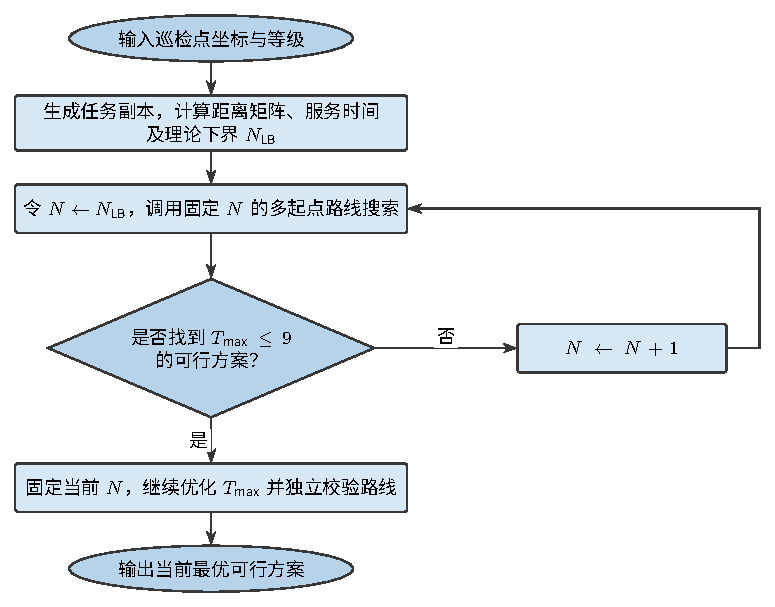
\includegraphics[
    width=0.84\textwidth,
    height=0.40\textheight,
    keepaspectratio
  ]{figures/q1_fleet_search_flowchart_revised.pdf}
  \caption{问题一无人机数量与路径的两阶段搜索流程}
  \label{fig:q1-fleet-flow}
\end{figure}
\FloatBarrier

\noindent\textbf{（2）路线优化与结果校验。}
在初始方案上，程序通过任务迁移、任务交换和 2-opt 构造邻域，并采用模拟退火搜索降低 \(T_{\max}\)。对使目标值增加 \(\Delta T>0\) 的候选方案，以概率

\begin{equation}
  P=\exp\left(-\frac{\Delta T}{\tau}\right)
  \label{eq:q1-sa-probability}
\end{equation}

予以接受，其中 \(\tau\) 为温度参数。退火结束后，再针对最长路线执行确定性平衡修复，并保留全部随机起点中 \(T_{\max}\) 最小的方案。若当前 \(N\) 找到满足 \(T_{\max}\leq9\) 的路线，则记录结果并继续优化；否则令 \(N\leftarrow N+1\)。最后独立复算各路线，检查巡检次数、同点连续访问、基地闭合和9小时限制，并将详细调度方案写入 \texttt{result1.xlsx}。固定无人机数量下的完整优化流程及相关源程序见附录B。

各算法操作的作用归纳于表~\ref{tab:q1-method-role}。

\begin{table}[H]
  \centering
  \caption{问题一各算法操作及其主要作用}
  \label{tab:q1-method-role}
  \begin{tabularx}{0.94\textwidth}{>{\centering\arraybackslash}p{3.2cm}X}
    \toprule
    算法操作 & 在本题中的主要作用 \\
    \midrule
    加权 K-means & 根据空间位置和巡检次数形成地理上较集中的初始任务区域 \\
    极角扫描 & 从不同方向切分任务点，增加初始路线结构的多样性 \\
    最近邻与 2-opt & 快速构造闭合路线并减少明显绕行和路线交叉 \\
    合法贪心插入 & 补充重复巡检任务，同时禁止同一物理点连续出现 \\
    任务迁移与交换 & 从最长路线向其他路线转移工作量，降低最大工作时间 \\
    模拟退火与多起点 & 接受少量劣化移动并重复搜索，降低陷入局部最优的可能性 \\
    确定性平衡修复 & 对当前最好方案进行最后的任务转移、交换和路线缩短 \\
    \bottomrule
  \end{tabularx}
\end{table}

\subsection{结果与解释}
按照赛题规定的展示格式，四个测试算例的无人机数量及单架无人机最长、最短工作时间见表~\ref{tab:q1-results}。

\begin{table}[H]
  \centering
  \caption{问题一无人机数量与完成时间计算结果}
  \label{tab:q1-results}
  \begin{tabularx}{0.98\textwidth}{c c >{\centering\arraybackslash}X >{\centering\arraybackslash}X}
    \toprule
    测试算例 & 无人机数量 $N$ & 单架无人机最长工作时间 $T_{\max}$（h） & 单架无人机最短工作时间 $T_{\min}$（h） \\
    \midrule
    Case 1 & 4 & 8.6111 & 8.5488 \\
    Case 2 & 2 & 7.5890 & 7.5775 \\
    Case 3 & 5 & 8.2876 & 8.2468 \\
    Case 4 & 4 & 8.6263 & 8.6058 \\
    \bottomrule
  \end{tabularx}
\end{table}

四个算例均满足 \(T_{\max}<9\text{ h}\)，说明表中方案能够在规定时间内完成全部巡检任务。理论分析得到 Case 1--Case 4 的无人机数量下界依次为3、2、4、4；其中 Case 2 和 Case 4 的计算数量与下界相等，可以确定 \(N_{\min}=2\) 和 \(N_{\min}=4\)。对于 Case 1 和 Case 3，当前结果分别给出4架和5架无人机的调度方案，但启发式算法在给定计算时间内未找到3架和4架方案并不等价于严格不可行，因此只能得到 \(3\leq N_{\min}\leq4\) 和 \(4\leq N_{\min}\leq5\)。此外，表中 \(T_{\max}\) 是多起点搜索得到的当前最好结果，未使用精确求解器证明其为固定 \(N\) 下的全局最优值。

\section{问题二的模型建立与求解}
\subsection{递进模型与均衡目标}

问题二完整继承问题一的任务副本集合、工作时间计算方法和路径可行性约束，包括每个任务副本恰好完成一次、无人机从基地出发并最终返回基地、同一物理巡检点禁止连续巡检、允许离开后再次返回以及单架无人机工作时间不超过9小时等约束。与问题一不同，问题二不再搜索无人机数量，而是固定

\begin{equation}
  N=N^{(1)},
  \qquad
  N^{(1)}=(4,2,5,4),
  \label{eq:q2-fixed-n}
\end{equation}

其中，向量各分量依次对应 Case 1--Case 4。鉴于 Case 1 和 Case 3 的当前数量尚未被严格证明为全局最少数量，本文将 \(N^{(1)}\) 表述为“问题一最终采用的无人机数量”，而不统一记作已经严格证明的 \(N_{\min}\)。

问题二不允许通过人为等待延长较短路线。均衡性改善只来源于任务副本重新分配和访问顺序调整，各无人机工作时间仍仅由飞行时间和有效巡检服务时间组成。主方案同时固定 $N=N^{(1)}$、取 $\varepsilon=0$，即不增加无人机、不放宽问题一当前完成时间，也不人为增加等待。

为刻画实际工作时间的均衡程度，定义

\begin{equation}
  T_{\max}=\max_{k\in K}T_k,
  \qquad
  T_{\min}=\min_{k\in K}T_k,
  \qquad
  \delta=T_{\max}-T_{\min}.
  \label{eq:q2-delta}
\end{equation}

由于恒有 \(T_{\max}\geq T_{\min}\)，题目中的绝对值可直接写成式~\eqref{eq:q2-delta}。车辆路径均衡问题中常以最长路线时间或最长、最短路线时间之差衡量工作负载差异\cite{matl2018,lehuedepeton2020}。本文采用“实际工作时间极差”，而不是任务数量差或飞行距离差。引入辅助变量 \(U,L\)，可将其线性表示为

\begin{equation}
\begin{aligned}
  U&\geq T_k, &&k\in K,\\
  L&\leq T_k, &&k\in K,\\
  \delta&=U-L.
\end{aligned}
\label{eq:q2-balance-variables}
\end{equation}

在最小化 \(\delta\) 时，最优解处有 \(U=T_{\max}\)、\(L=T_{\min}\)。但若只最小化极差，可能通过牺牲总体完成时间获得表面上的均衡。为保持问题一的优先目标，设

\begin{equation}
  C_{\mathrm{ref}}=T_{\max}^{(1)},
  \qquad
  T_{\max}^{(2)}\leq C_{\mathrm{ref}}+\varepsilon.
  \label{eq:q2-epsilon-constraint}
\end{equation}

主方案取 \(\varepsilon=0\)，即第二问的总体完成时间不得超过问题一当前最好可行方案。这相当于采用 \(\varepsilon\)-约束思想，在保持主要目标既有水平的条件下优化次级目标\cite{mavrotas2009}。四个算例的 \(C_{\mathrm{ref}}\) 依次为

\[
  (8.6111,\ 7.5890,\ 8.2876,\ 8.6263)\ \mathrm{h}.
\]

因此，前两问可以统一表示为

\begin{equation}
  \operatorname{lexmin}
  \left(
    N,T_{\max},\delta,\sum_{k\in K}T_k
  \right).
  \label{eq:q2-overall-objective}
\end{equation}

在第二问中，前两层已由式~\eqref{eq:q2-fixed-n} 和式~\eqref{eq:q2-epsilon-constraint} 固定，故对满足约束的候选方案采用

\begin{equation}
  F(S)=
  \left(
    \delta(S),T_{\max}(S),\sum_{k\in K}T_k(S)
  \right)
  \label{eq:q2-candidate-objective}
\end{equation}

进行词典序比较。总工作时间只作为前三项相同情况下的平局判别，以减少无效绕行。

\subsection{均衡优化算法}

程序直接读取问题一通过独立校验的调度方案 \(S^{(1)}\)，固定 \(N=N^{(1)}\) 并令 \(C_{\mathrm{ref}}=T_{\max}^{(1)}\)。每次迭代先按工作时间识别重载路线与轻载路线，再从重载路线向轻载路线迁移一个任务，或交换两条路线中的任务。发生改变的路线随后执行合法 2-opt，以消除明显绕行。候选方案必须同时满足巡检次数、基地闭合、同点不连续、9小时限制以及 \(T_{\max}\leq C_{\mathrm{ref}}\)，否则直接拒绝。

若候选方案的式~\eqref{eq:q2-candidate-objective} 词典序减小，则予以接受；对少量暂时劣化的方案按照模拟退火概率接受，以降低陷入局部最优的可能性。程序使用多个随机种子重复搜索，最后系统枚举重载路线与轻载路线间的单任务迁移，并对各路线充分执行 2-opt。上述过程不再改变无人机数量，也不重新构造问题一的任务副本模型，重点只在既有完成时间上界内重新分配真实巡检工作量。

需要特别说明的是，本文不允许无人机通过在基地、巡检点或航路中额外等待来增加工作时间。所有方案的等待时间均为0，\(T_k\) 只由实际飞行时间和有效巡检服务时间构成；路线调整后继续执行距离缩短操作。因此，均衡改善来自真实任务的重新分配和访问顺序优化，而不是人为延长短路线。该处理也避免了极差型非单调均衡指标可能诱发非必要绕行的问题\cite{matl2018}。

\subsection{计算结果与分析}

问题二的无人机数量、最大工作时间、最小工作时间和工作时间极差见表~\ref{tab:q2-results}。全部算例均使用问题一最终采用的无人机数量，且满足 \(T_{\max}^{(2)}\leq C_{\mathrm{ref}}<9\mathrm{h}\)。

\begin{table}[H]
  \centering
  \caption{问题二结果展示表}
  \label{tab:q2-results}
  \begin{tabularx}{0.98\textwidth}{c c >{\centering\arraybackslash}X >{\centering\arraybackslash}X >{\centering\arraybackslash}X}
    \toprule
    测试算例 & 无人机数量 $N$ & 单架无人机最长工作时间 $T_{\max}$（h） & 单架无人机最短工作时间 $T_{\min}$（h） & $\delta=|T_{\max}-T_{\min}|$（h） \\
    \midrule
    Case 1 & 4 & 8.6111 & 8.5937 & 0.0174 \\
    Case 2 & 2 & 7.5841 & 7.5737 & 0.0103 \\
    Case 3 & 5 & 8.2824 & 8.2586 & 0.0238 \\
    Case 4 & 4 & 8.6197 & 8.6120 & 0.0077 \\
    \bottomrule
  \end{tabularx}
\end{table}

为量化均衡改善效果，记问题一、问题二的工作时间极差分别为 \(\delta_1,\delta_2\)，定义极差下降量和下降比例为

\begin{equation}
  \Delta\delta=\delta_1-\delta_2,
  \qquad
  \eta_{\delta}=\frac{\delta_1-\delta_2}{\delta_1}\times100\%.
  \label{eq:q2-delta-reduction}
\end{equation}

计算结果见表~\ref{tab:q2-comparison}。

\begin{table}[H]
  \centering
  \caption{问题一与问题二工作时间极差对比}
  \label{tab:q2-comparison}
  \begin{tabular}{cccc}
    \toprule
    测试算例 & $\delta_1$/min & $\delta_2$/min & 下降比例 \\
    \midrule
    Case 1 & 3.74 & 1.04 & 72.1\% \\
    Case 2 & 0.69 & 0.62 & 9.7\% \\
    Case 3 & 2.45 & 1.43 & 41.8\% \\
    Case 4 & 1.23 & 0.46 & 62.6\% \\
    \bottomrule
  \end{tabular}
  \par\smallskip
  \parbox{0.78\textwidth}{\footnotesize 注：极差及下降比例均由程序输出的未舍入数据计算，表中分钟数仅作显示舍入。}
\end{table}

\begin{figure}[H]
  \centering
  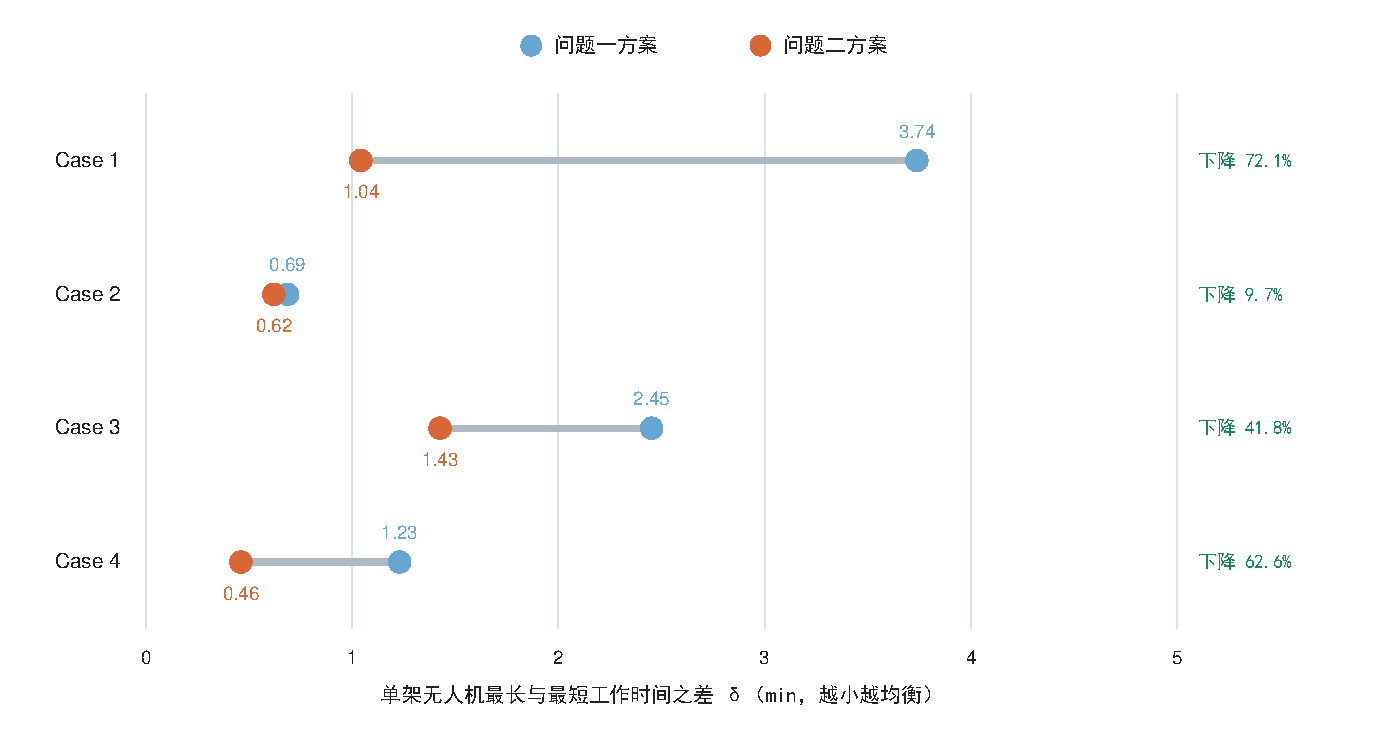
\includegraphics[width=0.94\textwidth]{generated_figures/q2_balance_improvement_dumbbell.pdf}
  \caption{问题一与问题二工作时间极差对比}
  \label{fig:q2-workload-comparison}
\end{figure}

由表~\ref{tab:q2-comparison} 和图~\ref{fig:q2-workload-comparison} 可见，问题二所得方案在保持无人机数量不变的基础上，进一步缩小了不同无人机之间的工作时间极差。按照程序输出的未舍入数据计算，Case 1、Case 3 和 Case 4 的极差分别下降72.1\%、41.8\%和62.6\%；Case 2 在问题一中已经较为均衡，极差仍由约0.69分钟下降至0.62分钟，下降9.7\%。优化后四个算例的工作时间极差均不超过1.43分钟，说明所构造方案具有较好的负载均衡性。与此同时，Case 2--Case 4 的 \(T_{\max}\) 还略有下降，Case 1 保持原完成时间上界，说明均衡改善没有以牺牲总体完成时间为代价。

正文不逐行展开较长的巡检点序列。四个算例中每架无人机的基地闭合路线、飞行距离、巡检次数和工作时间均保存在支撑材料 \texttt{result2.xlsx}，可复算的完整结构化路线保存在 \texttt{q2\_solution.json}；相应程序入口为 \texttt{q2\_solver.py}。

\section{问题三的模型建立与求解}
\subsection{模型建立}

问题三并非管制信息随机到达的在线调度，而是在管制区域及其生效时段均预先已知的条件下，对前两问模型增加绝对时刻和时变通行约束，属于确定性时间依赖路径问题\cite{gendreau2015time}。题目未明确说明第三问是否允许重新配置无人机数量；若将机队规模视为不受约束的决策变量，而目标仅为缩短完成时间，则会产生不断增加无人机的退化倾向。为保持三问的递进关系，本文将问题一最终采用的机队规模视为系统已有配置，正式方案固定为 $N_0=(4,2,5,4)$。这是本文用于消除题意歧义的建模约定，并非题目明文规定；增加无人机的结果仅用于第8节敏感性分析。

任务副本、巡检次数、基地往返以及同一物理点不得连续巡检等约束保持不变。以8:00为 $t=0$，若附件钟表时刻为 $h{:}m$，则相对时刻按 $t_{\mathrm{rel}}=60(h-8)+m$ 换算，例如 $8{:}00\mapsto0$、$10{:}30\mapsto150$、$17{:}00\mapsto540$。问题一中的9小时限制只用于确定机队规模，问题三原文未再次规定任务必须在9小时内完成，因此本文不将17:00作为任务截止时刻。17:00仅表示相关动态管制区在该时刻解除，无人机可以在此后继续执行巡检任务并返回基地。

将第 $r$ 个动态圆形管制区记为 $Z_r=(\boldsymbol c_r,R_r,[\alpha_r,\beta_r))$。其中 $\boldsymbol c_r$、$R_r$ 分别为圆心和半径。时间窗采用左闭右开的半开区间：开始时刻 $\alpha_r$ 计入管制，结束时刻 $\beta_r$ 不再计入，从而避免端点重复判定。Case 4 中 $Z_8$ 的开始和结束时刻均为17:00，故其时间窗为 $[540,540)=\varnothing$，不产生实际管制约束；本文不将其解释为“从17:00持续至任务结束”，也不人为补充管制时长。对航段 $(i,j)$，设正常飞行时间为 $\tau_{ij}$，程序解析求得该线段进入、离开圆 $r$ 的参数 $\lambda_{ijr}^{-}$ 与 $\lambda_{ijr}^{+}$。模型中的核心时空约束及通行函数集中写为

\begin{equation}
\begin{aligned}
 \boldsymbol p_{ij}(\lambda)&=\boldsymbol p_i+\lambda(\boldsymbol p_j-\boldsymbol p_i),\quad 0\leq\lambda\leq1,\\
 t+\lambda\tau_{ij}\in[\alpha_r,\beta_r)&\ \Longrightarrow\ 
 \|\boldsymbol p_{ij}(\lambda)-\boldsymbol c_r\|_2>R_r,\\
 \mathcal F_{ijr}&=[\alpha_r-\lambda_{ijr}^{+}\tau_{ij},\,\beta_r-\lambda_{ijr}^{-}\tau_{ij}),
 \quad \mathcal F_{ij}=\bigcup_r\mathcal F_{ijr},\\
 D_{ij}(t)&=\min\{s\geq t:s\notin\mathcal F_{ij}\},\quad
 A_{ij}(t)=D_{ij}(t)+\tau_{ij}.
\end{aligned}
\label{eq:q3-core-dynamic}
\end{equation}

式~\eqref{eq:q3-core-dynamic} 表明，一条直线航段在几何上穿过管制圆并不意味着必然违规；只有无人机通过圆内部分的实际时间与管制窗重叠时，才形成时空冲突。当同一航段受多个管制圆影响时，程序将各圆产生的非空禁用区间按开始时刻排序，合并相交或相邻区间后组成 $\mathcal F_{ij}$，再从计划时刻起寻找第一个不属于该集合的出发时刻 $D_{ij}(t)$。

服务过程同样受动态管制约束。设任务 $i$ 的服务开始时刻为 $s_i$、服务时间为 $t_s=5$ min；若 $\|\boldsymbol p_i-\boldsymbol c_r\|_2\leq R_r$，必须满足 $[s_i,s_i+t_s)\cap[\alpha_r,\beta_r)=\varnothing$，即完整5分钟服务区间均须安全，不能只检查到达或服务开始时刻。若原计划航段当前不可通行，则推迟至最早可行出发时刻；若当前节点在计划等待区间内也不安全，则沿既定访问序列向前回溯，将等待前移至最近一个能在整个区间保持安全的已访问节点，并重新递推后续时刻。问题三只允许这种满足管制要求所必需的等待，不允许为了减小 $\delta$ 任意延长短路线；等待时间计入工作时间，在基地等待也从8:00开始计时。图~\ref{fig:q3-principle} 给出了这一联合判定过程。

\begin{figure}[H]
  \centering
  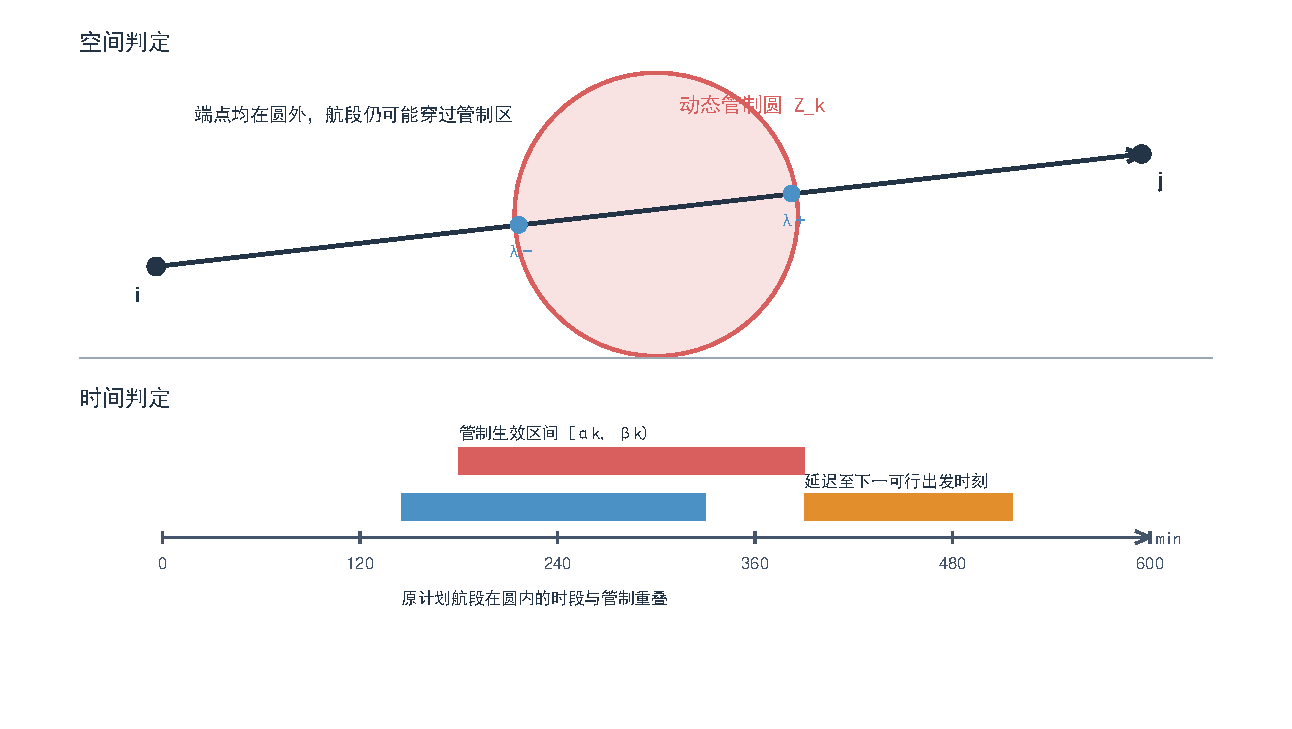
\includegraphics[width=0.90\textwidth]{generated_figures/q3_spatiotemporal_principle.pdf}
  \caption{航段与动态圆形禁飞区的时空耦合判定}
  \label{fig:q3-principle}
\end{figure}

设无人机 $k$ 的节点序列为 $(v_{k,0},\ldots,v_{k,m_k})$，从8:00开始递推到达、服务和离开时刻。其工作时间由实际飞行、有效巡检和必要安全等待组成。由于 $T_k^{\mathrm{fly}}$、$T_k^{\mathrm{service}}$ 以小时计而 $T_k^{\mathrm{wait}}$ 以分钟计，故 $T_k=T_k^{\mathrm{fly}}+T_k^{\mathrm{service}}+T_k^{\mathrm{wait}}/60$。并记 $T_{\max}=\max_kT_k$、$T_{\min}=\min_kT_k$、$\delta=T_{\max}-T_{\min}$。对需要重复巡检的点，程序为每次巡检建立唯一任务副本，从而保证移动、交换后仍能逐一核对任务次数。

\subsection{求解方法}

\noindent\textbf{直飞--等待基准算法A。}

算法A首先读取问题二已通过校验的路线，解析计算直线航段与各管制圆的相交参数及禁用出发区间。给定任务序列后，内层评价器按照访问顺序递推最早可行时刻：航段若在管制生效时穿圆，则在最近的安全节点等待至直飞可行；若目标点的5分钟服务区间与管制窗冲突，则同样将必要等待前移。算法A不增设圆边界绕飞节点，其空间避让依靠调整访问顺序和跨无人机重分配实现，因此属于“直飞--必要等待”的快速基准方法。

外层在任务迁移、跨路线交换和路线片段反转等邻域之间切换，并用多起点模拟退火跳出局部最优，候选解按 $(T_{\max},\delta,\sum_kT_k)$ 的字典序更新。数值计算中每个算例使用5个随机起点，每个起点最多迭代25000次；温度由0.12逐步降至0.002。完成全部随机起点或达到每个算例35秒总时间预算时停止，并输出当前搜索范围内的最好可行方案。算法A的作用是提供稳定、可复算的比较基准，而不是填写第三问的最终表格。

\begin{figure}[H]
  \centering
  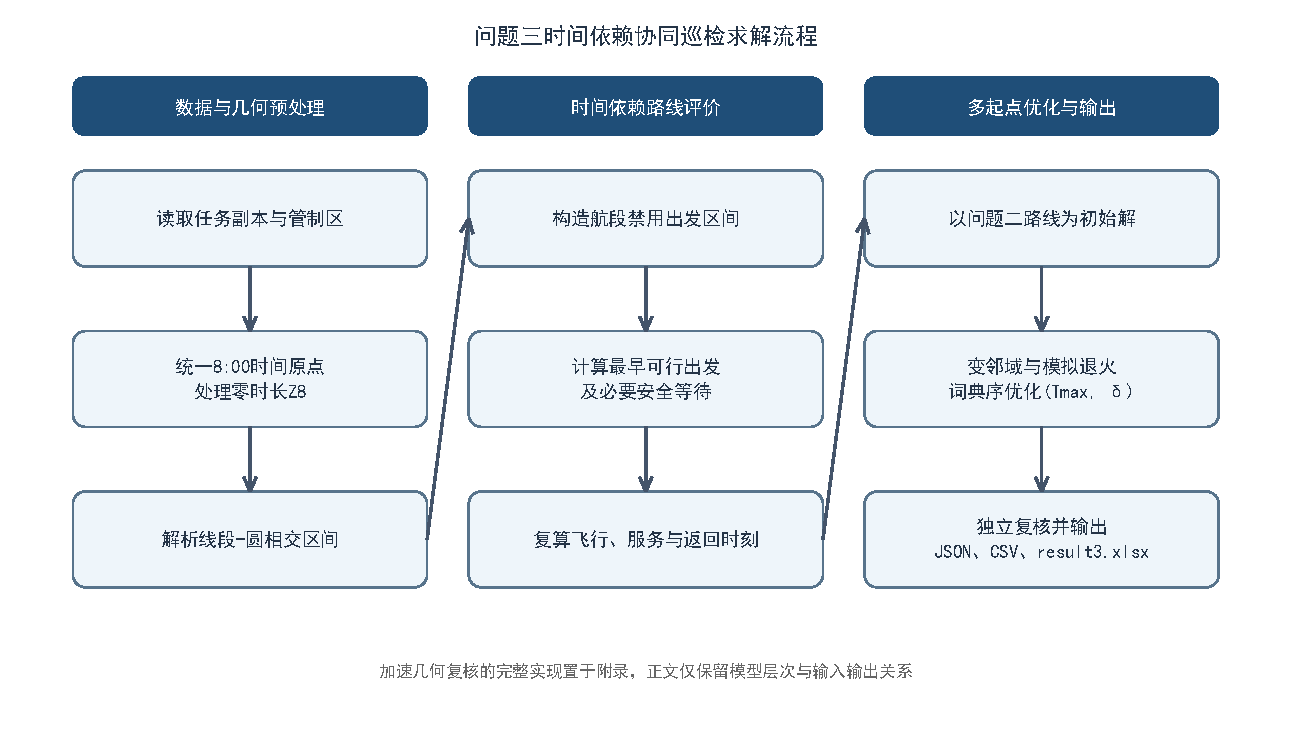
\includegraphics[width=0.90\textwidth]{generated_figures/q3_solver_flowchart.pdf}
  \caption{基准算法A的时间依赖路线求解流程}
  \label{fig:q3-solver-flow}
\end{figure}

\medskip
\noindent\textbf{时变可见图两阶段算法B。}

算法B保留算法A的解析冲突检查和最早时刻递推，并在航段评价中增加空间绕飞选择。记 $n_b$ 为每个有效管制圆的外偏候选节点数，本次取 $n_b=16$；$\rho$ 为附加安全裕度，本次取 $\rho=0$；$\widehat R_r$ 为外偏采样半径。为避免候选节点落在原禁飞边界上，并防止相邻采样点之间的弦切入圆内，程序采用 $\widehat R_r=(R_r+\rho)\sec(\pi/n_b)+10^{-6}$。即使 $\rho=0$，几何外偏量 $R_r[\sec(\pi/16)-1]+10^{-6}$ 仍为正。

本文将管制圆视为闭圆盘，圆周边界同样属于管制区域；几何判断对判别式和点到线段距离采用统一数值容差，相切按接触管制圆处理。候选节点仅用于构造时变可见图，任意两节点间的可见边仍须在原半径 $R_r$ 下通过解析线段--圆盘检查，不满足安全条件的边均予删除。算法同时比较“安全等待后直飞”和“沿外偏节点改道”两类通行方式，并对最终折线路径的每一小段重新进行时空联合验证。由于时变可见图只使用有限个外偏节点，所得路线是连续圆障碍最短路的离散近似，本文不声称其为连续空间中的全局最短路径。

外层搜索除迁移、交换和片段反转外，还加入跨路线片段交换，并将问题二路线、算法A路线及随机扰动路线共同作为初始解。为体现总体完成时间优先，并允许在近似最优效率范围内进一步改善负载均衡性，算法B采用基于 $\varepsilon$-约束的近似字典序两阶段准则

\begin{equation}
\begin{aligned}
T_{\max}^{B,*}&=\min_{S\in\Omega_3(N_0)}T_{\max}(S),\\
\min_{S\in\Omega_3(N_0)}\;&\left(\delta(S),\sum_kT_k(S)\right)
\quad\text{s.t.}\quad T_{\max}(S)\leq(1+\varepsilon_T)T_{\max}^{B,*},
\end{aligned}
\qquad \varepsilon_T=0.005 .
\label{eq:q3-two-stage}
\end{equation}

其中 $\Omega_3(N_0)$ 表示固定机队规模且满足全部巡检、基地闭合和动态禁飞约束的可行方案集合。本文取 $\varepsilon_T=0.005$，表示均衡优化只允许总体完成时间相对第一阶段当前最好值增加不超过0.5\%，从而给效率损失设置直观且较严格的上界；该参数是效率与均衡之间的建模取舍，不是数值误差。第二阶段若发现更小的 $T_{\max}$，则立即回代更新 $T_{\max}^{B,*}$ 并重新执行均衡搜索，使效率阈值始终以当前最好完成时间为基准。每个阶段最多迭代1200次，基础搜索每个“算例--机队规模”采用30秒预算；回代最多追加3轮，每轮最多10秒。达到迭代或时间上限，或回代后未再发现更小的 $T_{\max}$ 时停止。最终结果均称为“当前搜索范围内最好可行方案”，不声称已经证明全局最优。

\begin{table}[H]
  \centering
  \caption{算法A与算法B的求解机制比较}
  \label{tab:q3-method-comparison}
  \small
  \begin{tabularx}{0.94\textwidth}{c >{\centering\arraybackslash}X >{\centering\arraybackslash}X}
    \toprule
    比较内容 & 算法A & 算法B \\
    \midrule
    航段方式 & 直飞或安全等待 & 直飞、安全等待或空间绕飞 \\
    几何结构 & 原任务节点 & 原任务节点与圆外偏置节点 \\
    动态评价 & 禁用出发区间与时刻递推 & 时变可见图与逐段时刻递推 \\
    初始解 & 问题二路线 & 问题二路线、算法A路线及随机扰动 \\
    邻域操作 & 迁移、交换、反转 & 增加跨路线片段交换 \\
    优化准则 & 字典序基准搜索 & $\varepsilon$-约束两阶段优化 \\
    论文作用 & 对照基准 & 固定 $N_0$ 的正式方案 \\
    \bottomrule
  \end{tabularx}
\end{table}

\subsection{计算结果与分析}

按照上述约定，第三问正式结果采用算法B在固定机队规模 $N_0=N^{(1)}=(4,2,5,4)$ 下得到的均衡方案，列于表~\ref{tab:q3-results}；该表用于填写赛题所给表4。算法A仅作为基准方法，不同机队规模结果仅作为敏感性分析。表中工作时间从8:00起算，允许在17:00后继续执行任务并返回基地。

\begin{table}[H]
  \centering
  \caption{问题三结果展示表（算法B固定 $N_0$ 的正式方案）}
  \label{tab:q3-results}
  \begin{tabularx}{0.98\textwidth}{c c >{\centering\arraybackslash}X >{\centering\arraybackslash}X >{\centering\arraybackslash}X}
    \toprule
    测试算例 & 无人机数量 $N$ & 单架无人机最长工作时间 $T_{\max}$（h） & 单架无人机最短工作时间 $T_{\min}$（h） & $\delta=|T_{\max}-T_{\min}|$（h） \\
    \midrule
    Case 1 & 4 & 8.6111 & 8.5937 & 0.0174 \\
    Case 2 & 2 & 13.1404 & 13.1401 & 0.0003 \\
    Case 3 & 5 & 9.6280 & 9.5822 & 0.0458 \\
    Case 4 & 4 & 10.9250 & 10.8597 & 0.0652 \\
    \bottomrule
  \end{tabularx}
\end{table}

表中工作时间以小时表示并保留4位小数，最晚返回时刻则根据程序保存的未舍入秒级结果计算，因此直接使用表中四舍五入后的小时数换算时可能出现约1秒差异。

\begin{table}[H]
  \centering
  \caption{固定 $N_0$ 时算法A与算法B的结果对比}
  \label{tab:q3-ab-comparison}
  \small
  \begin{tabularx}{0.98\textwidth}{c c *{5}{>{\centering\arraybackslash}X}}
    \toprule
    算例 & $N_0$ & $T_{\max}^{A}$/h & $T_{\max}^{B,*}$/h & $T_{\max}^{B}$/h & $\delta^{A}$/h & $\delta^{B}$/h \\
    \midrule
    Case 1 & 4 & 8.6111 & 8.6111 & 8.6111 & 0.0174 & 0.0174 \\
    Case 2 & 2 & 13.3779 & 13.1404 & 13.1404 & 0.0146 & 0.0003 \\
    Case 3 & 5 & 9.6086 & 9.6086 & 9.6280 & 0.1237 & 0.0458 \\
    Case 4 & 4 & 10.8711 & 10.8711 & 10.9250 & 0.6808 & 0.0652 \\
    \bottomrule
  \end{tabularx}
\end{table}

表~\ref{tab:q3-ab-comparison} 中 $T_{\max}^{B,*}$ 为算法B第一阶段得到的效率基准，$T_{\max}^{B}$ 为第二阶段均衡后的正式值。Case 1 未发生实际管制冲突，两种算法结果一致。Case 2 中，空间绕飞与任务重排使完成时间由13.3779小时降至13.1404小时，必要等待由189.297分钟降至47.645分钟，同时极差降至约0.02分钟。Case 3、Case 4 的第二阶段分别在第一阶段最好完成时间上增加约0.20\%和0.50\%，均未超过0.5\%阈值，而极差分别缩小约63.0\%和90.4\%。这说明在严格限制效率损失后，算法B能显著改善固定机队下的工作负载均衡。

\begin{table}[H]
  \centering
  \caption{固定 $N_0$ 时必要等待与绕行结果对比}
  \label{tab:q3-wait-detour}
  \begin{tabular}{c c c c}
    \toprule
    算例 & 算法A必要等待/min & 算法B必要等待/min & 算法B绕行航段数 \\
    \midrule
    Case 1 & 0.000 & 0.000 & 0 \\
    Case 2 & 189.297 & 47.645 & 12 \\
    Case 3 & 59.023 & 19.671 & 1 \\
    Case 4 & 0.000 & 0.000 & 1 \\
    \bottomrule
  \end{tabular}
\end{table}

表~\ref{tab:q3-wait-detour} 进一步表明，算法B并非单纯依靠延后任务改善可行性，而是利用空间绕行替代部分长时间等待。需要说明的是，两种算法的邻域规模、单次评价成本和总计算预算并不完全相同，因此表~\ref{tab:q3-ab-comparison}、\ref{tab:q3-wait-detour} 主要比较在本文既定求解流程下获得的最终方案质量，不把运行时间差异作为搜索效率优劣的严格证据。

\begin{figure}[H]
  \centering
  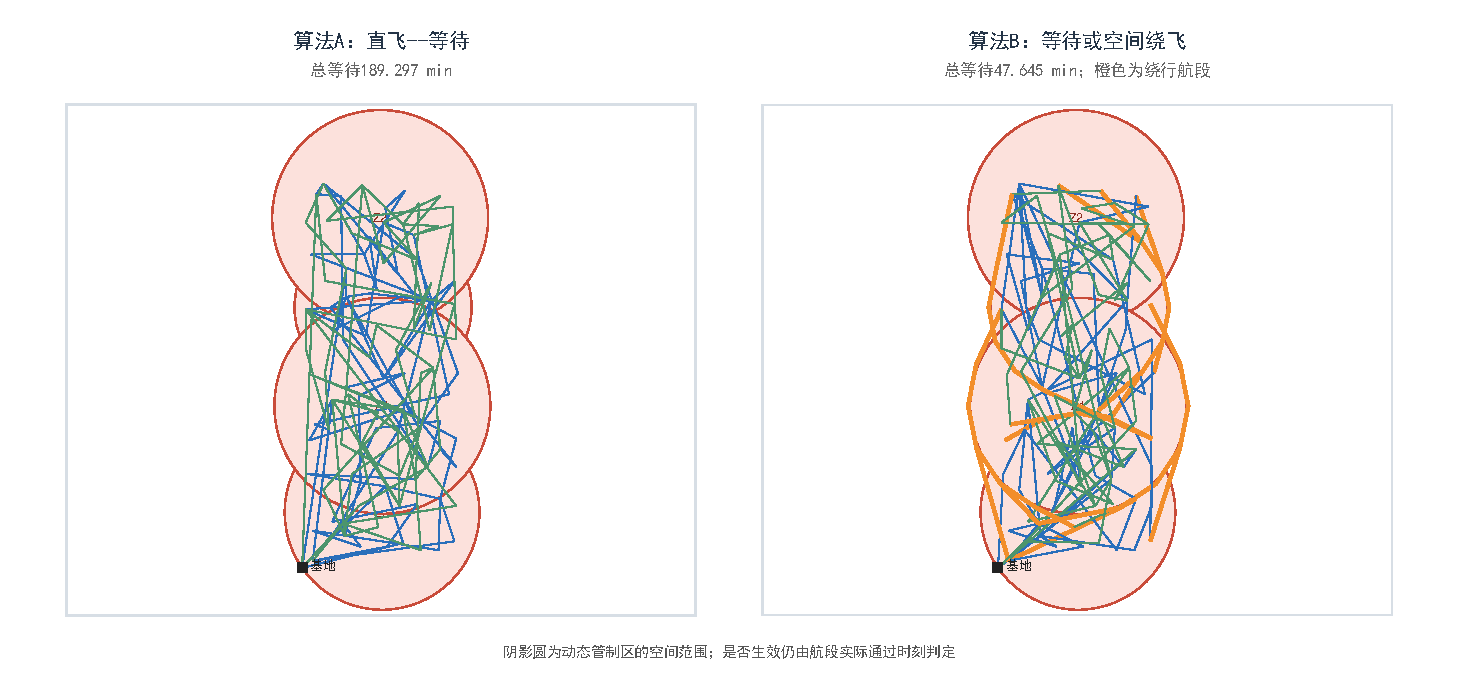
\includegraphics[width=\textwidth]{generated_figures/q3_case2_ab_routes.pdf}
  \caption{Case 2中算法A与算法B的实际航迹对比（算法B橙色折线为绕行组成航段）}
  \label{fig:q3-case2-ab-routes}
\end{figure}

图~\ref{fig:q3-case2-ab-routes} 由两套程序的已验证逐事件结果直接绘制。阴影圆表示管制区的空间范围，实际冲突仍由飞行通过时刻与管制时间窗联合判断；因此算法A的直线航迹在空间上穿圆并不必然违规，而是在时间冲突发生时等待后再通过。算法B则对其中部分冲突航段采用圆外折线，从而显著降低累计等待。

正式方案中，Case 1--Case 4 的最晚返回时刻依次为16:36:39、21:08:25、17:37:40和18:55:29。Case 3 和 Case 4 在均衡阶段主动利用很小的完成时间容差换取更紧凑的工时分布；该取舍已由式~\eqref{eq:q3-two-stage} 明确限定，不属于任意增加等待。

算法B的正式路线、逐事件时间表和12组敏感性结果保存于支撑材料 \texttt{result3.xlsx}，可复算的结构化结果保存于 \texttt{q3\_solution.json}；算法A的对照结果分别另存为 \texttt{result3\_algorithmA.xlsx} 和 \texttt{q3\_solution\_algorithmA.json}，避免两套程序和结果混淆。

\section{模型检验与敏感性分析}
针对前两问，本文采用“求解程序生成结果、独立校验器重新读取原始附件并复算”的方式检查结果一致性。校验器逐条检查基地是否只出现于路线首尾、同一物理点是否连续出现、I/II/III级巡检点是否分别完成3/2/1次有效巡检，并根据

\[
  T_k=\frac{D_k}{55}+\frac{m_k}{12}
\]

重新计算每架无人机的工作时间。其中，\(D_k\) 为实际飞行距离，\(m_k\) 为有效巡检次数。问题二还额外检查 \(N=N^{(1)}\)、等待时间为0以及 \(T_{\max}^{(2)}\leq T_{\max}^{(1)}+\varepsilon\)。四个算例均通过上述检查，JSON 与 Excel 汇总值和逐路线复算值一致。

问题二主结果取 \(\varepsilon=0\)，这是对“保证总体完成时间尽可能短”的保守解释。当 \(\varepsilon>0\) 时，可允许极小的总体完成时间损失来换取进一步的均衡改善；但由于当前四个算例已经将极差控制在约1.43分钟以内，本文不在主结果中放宽该参数。

\subsection{问题三独立可行性检验}

问题三另由独立程序重新读取原始附件，并逐事件复核唯一任务副本、基地闭合、时间连续性、每条折线航段的穿圆时段、管制区内服务和非基地安全等待，同时核对 $T_{\max}$、$T_{\min}$、$\delta$ 及两阶段效率阈值。算法B在4个算例、每个算例3种机队规模下形成的12组结果全部通过验证。该结论证明输出方案满足程序所实现的全部约束，但不等同于对全局最优性的证明。算法B的逐事件独立验证程序和算法A的快速解析校验程序见附录D。

\clearpage
\subsection{问题三机队规模敏感性}

为考察题目对无人机数量未作明确限制时的结果变化，本文另取 $N=N_0,N_0+1,N_0+2$ 运行算法B。表~\ref{tab:q3-fleet-sensitivity} 仅用于敏感性分析，不替代表~\ref{tab:q3-results} 的固定 $N_0$ 正式方案。

\begin{table}[H]
  \centering
  \caption{算法B在不同机队规模下的敏感性结果}
  \label{tab:q3-fleet-sensitivity}
  \scriptsize
  \begin{tabularx}{0.99\textwidth}{c c *{5}{>{\centering\arraybackslash}X}}
    \toprule
    算例 & $N$ & $T_{\max}^{*}$/h & $T_{\max}$/h & $\delta$/h & 总等待/min & 单机最大等待/min \\
    \midrule
    Case 1 & 4 & 8.6111 & 8.6111 & 0.0174 & 0.000 & 0.000 \\
    Case 1 & 5 & 8.5270 & 8.5270 & 0.0615 & 0.000 & 0.000 \\
    Case 1 & 6 & 8.3513 & 8.3513 & 0.0732 & 0.000 & 0.000 \\
    Case 2 & 2 & 13.1404 & 13.1404 & 0.0003 & 47.645 & 34.612 \\
    Case 2 & 3 & 11.9325 & 11.9436 & 0.0081 & 448.214 & 233.441 \\
    Case 2 & 4 & 11.0787 & 11.0969 & 0.0108 & 952.904 & 269.184 \\
    Case 3 & 5 & 9.6086 & 9.6280 & 0.0458 & 19.671 & 19.671 \\
    Case 3 & 6 & 9.5855 & 9.6241 & 0.0778 & 2.117 & 2.117 \\
    Case 3 & 7 & 9.4650 & 9.4650 & 0.1435 & 0.000 & 0.000 \\
    Case 4 & 4 & 10.8711 & 10.9250 & 0.0652 & 0.000 & 0.000 \\
    Case 4 & 5 & 10.7858 & 10.7858 & 0.0169 & 1.048 & 1.048 \\
    Case 4 & 6 & 10.6692 & 10.6692 & 0.0183 & 3.216 & 3.216 \\
    \bottomrule
  \end{tabularx}
\end{table}

总体上，当前搜索得到的 $T_{\max}$ 随机队规模增加而下降，其中 Case 2 对增加无人机最敏感：由2架增加至3架和4架后，完成时间分别再缩短约71.8分钟和50.8分钟。表中的总等待是所有无人机等待时间之和，而 $T_{\max}$ 只由最晚返回的一架无人机决定；增机后更多并行路线进入管制时间窗，等待分散在多架无人机上，因而总等待增加并不必然导致系统完成时间增加。Case 2 的单机最大等待虽由34.612分钟增至233.441分钟和269.184分钟，但并行作业仍使最后返回时刻显著提前。$\delta$ 并不随 $N$ 单调变化，这是两阶段效率阈值、任务离散性和启发式搜索共同作用的结果。由于题目没有给出新增无人机成本或数量上限，不能仅凭该表定义无条件的“最优机队规模”，故仍以固定 $N_0$ 的方案作为正式答案。

\section{模型评价与推广}
\subsection{模型优点}

\begin{enumerate}[label=（\arabic*）]
  \item \textbf{三问之间具有统一且递进的模型结构。}本文将不同等级巡检点的次数要求展开为相互独立的任务副本，在统一框架下依次研究机队规模、系统完成时间和负载均衡问题。问题三继续沿用前两问的任务副本、路线结构和时间计算方法，仅进一步引入具有生效时段的圆形禁飞区，实现了从静态多无人机路径规划到时空耦合路径规划的自然扩展。

  \item \textbf{动态禁飞约束的处理较为完整。}问题三以当天8:00为统一时间原点，根据无人机到达各节点的绝对时刻，判断航段飞行、圆内巡检和原地等待是否与管制时间发生冲突。模型不仅检查巡检点是否位于禁飞区内，还对每条航段进行线段与圆形区域的相交计算，避免只检查航段端点而遗漏中途穿越禁飞区的情况。对于 Case 4 中的异常记录 Z8，统一按照半开区间 $[17{:}00,17{:}00)=\varnothing$ 处理，使数据异常的解释明确且可复现。

  \item \textbf{优化目标的优先级与题意一致。}本文首先在给定机队规模下最小化系统完成时间 $T_{\max}$，再在 $T_{\max}\leq(1+\varepsilon_T)T_{\max}^{*}$ 的限制下最小化工作时间极差 $\delta=T_{\max}-T_{\min}$。这种两阶段方法避免了简单加权和中权重难以解释的问题，也限制了为追求负载均衡而产生的效率损失。算法A采用直飞与安全等待相结合的方式，适用于管制稀疏或持续时间较短的情形；算法B进一步比较空间绕飞与时间等待，适用于绕飞收益较明显的管制情形。

  \item \textbf{模型结果能够独立复核。}独立校验器从附件原始数据重新读取巡检需求和管制信息，逐架无人机、逐个任务和逐条航段复算任务覆盖次数、路线连续性、飞行时间、巡检时间及禁飞约束。因此，论文模型、程序结果和输出文件之间可以相互核对。需要说明的是，校验器能够确认方案满足约束，但不能据此证明方案达到全局最优。
\end{enumerate}

\subsection{模型不足与改进}

\begin{enumerate}[label=（\arabic*）]
  \item \textbf{有限计算结果尚不能代替全局最优性证明。}本文得到的是给定算法、参数和计算时间内的最好可行方案。以 Case 1 使用3架无人机为例，12个随机起点并行运行约6小时后，最好结果为 $T_{\max}=10.3195$ h，其余结果也大多集中在 $10.32\sim10.50$ h。这说明现有算法容易收敛到相似的局部最优区域，也表明将结果继续压缩至9小时具有较大困难。但是，这些搜索过程使用相近的构造方法和邻域算子，不能被视为相互独立的随机试验。因此，6小时内没有找到可行解只能作为“3架完成任务较为困难”的计算证据，不能严格证明3架无人机不可行，论文中仍应保留 $3\leq N_{\min}\leq4$ 的结论。

  \item \textbf{圆形障碍绕行仍存在离散近似。}算法B取 $n_b=16$，相邻边界采样点的圆周角为 $360^{\circ}/16=22.5^{\circ}$，是在可见图规模和绕行精度之间作出的折中。虽然外偏半径能够保证所构造的离散绕行边不进入原禁飞圆，但连续空间中的最短绕行路径仍被有限个边界节点近似。增加 $n_b$ 可以提高空间分辨率，同时也会增加可见图的节点数、候选边数和时间依赖最短路的计算量。后续可比较 $n_b\in\{8,16,32\}$ 时的完成时间、总航程和运行时间，或使用解析切线、圆弧连接及局部自适应加密方法减小离散误差\cite{debnath2024}。

  \item \textbf{负载均衡参数和机队规模仍带有工程取舍。}本文取 $\varepsilon_T=0.005$，即允许第二阶段方案的最大完成时间相对第一阶段最优值增加不超过0.5\%。该参数保证了效率优先，但其具体取值仍可通过 $\varepsilon_T\in\{0,0.001,0.0025,0.005\}$ 的敏感性试验进一步验证。与此同时，极差 $\delta$ 只由工作时间最长和最短的两架无人机决定，不能完整描述其余无人机的负载分布，因此可补充报告标准差或变异系数，但不再将其加入主优化目标。此外，如果允许无人机数量无限增加而不考虑使用成本，单纯最小化 $T_{\max}$ 会使模型倾向于不断扩充机队，后续可通过边际收益曲线或增加机队投入成本确定更加合理的无人机数量。

  \item \textbf{算法仍有进一步改进空间。}针对现有搜索容易停留在10.3 h附近的问题，可将目标调整为优先减少超过9小时的部分，并从当前最好结果开始逐步压缩时间门槛。局部搜索方面，可采用 ALNS 重点破坏瓶颈路线，并加入 2-opt$^{*}$、Or-opt、Cross-exchange 和 Ejection chain 等跨路线邻域\cite{ropke2006alns}；同时利用混合遗传搜索维持解的多样性，在交叉和变异后再进行任务修复与局部强化\cite{vidal2012,vidal2022}。并行计算也可由相互独立的随机起点改为异构岛模型，使不同进程分别运行 ALNS、模拟退火和混合遗传搜索，并通过精英解池交换优质方案。

  如果需要严格判定3架无人机能否在9小时内完成任务，则还需借助精确算法。一种可行思路是先生成工作时间不超过9小时的单机路线，再建立集合划分模型，判断能否选择3条路线完整覆盖全部任务副本，并进一步采用列生成和分支定价方法闭合上下界\cite{feillet2010,costa2019}。启发式算法负责尽可能改进可行解上界，精确算法负责计算下界或给出不可行性证明，两者结合才能更可靠地判断最小机队规模。

  \item \textbf{模型对实际飞行环境仍作了确定性简化。}本文假设无人机速度恒定、管制信息在任务开始前完全已知，并忽略电量消耗、风速变化、通信延迟和无人机之间的空中冲突。若用于实际巡检，还需要加入续航与返航电量约束，并在管制区域临时新增、提前结束或延长时采用滚动时域方法，根据无人机当前位置和剩余任务重新规划路径\cite{adamo2024}。
\end{enumerate}

% =============================================================
% 参考文献采用 GB/T 7714—2015 顺序编码制，由 references.bib 统一生成。
% =============================================================
\clearpage
\section*{参考文献}
\bibliographystyle{gbt7714-numerical}
\bibliography{references}

% =============================================================
% AI 使用说明：位于参考文献之后，并按专项规定如实填写。
% =============================================================
\clearpage
\section*{人工智能工具使用说明}

本队与AI工具的交互以“在队员已有思路和程序基础上进行辅助整理、检查与润色”为主。典型提示词及完整交互记录已存档，详见附录文件。

\noindent 对AI输出的采纳、人工修改和核验情况如下：

\begin{enumerate}[label=\arabic*.]
  \item 所有AI输出\textbf{仅作为辅助参考}，核心决策（变量定义、约束逻辑、算法参数、停止条件、结果判定）均由队员根据实际程序和题目条件独立确定。
  \item 对表述类输出：逐句比对后进行大幅删改、重写或补充，确保与程序和计算结果完全一致。
  \item 对代码类输出：仅用于解释、补充注释或调试建议，最终程序全部由队员实际编写、运行并独立验证。
  \item 对图表与表格：AI生成初稿或代码后，队员重新计算数值、调整图例与单位、核对正文引用。
  \item 语言润色部分：仅采纳符合原意的修改，其余全部人工重写。
  \item 最终论文、程序、结果文件及支撑材料均经全体队员人工审阅、复算并共同确认，对原创性、真实性与准确性负全部责任。
\end{enumerate}

\noindent\textbf{郑重声明：}本参赛队确保核心建模与分析由队员主导，AI工具仅用于上述辅助环节。所有AI参与完成的内容均已逐项人工审查与核实。

% =============================================================
% 附录：与正文共用同一 TeX 文件，页码自然连续。
% =============================================================
\clearpage
\appendix
\linespread{1.25}\selectfont
\Urlmuskip=0mu plus 1mu
\renewcommand{\thesection}{\Alph{section}}
\renewcommand{\thesubsection}{\Alph{section}.\arabic{subsection}}
\titleformat{\section}{\centering\bfseries\fontsize{15pt}{20pt}\selectfont}
  {附录\thesection\quad}{0pt}{}

\section{支撑材料文件列表}

支撑材料以 ZIP 压缩包单独提交。为便于评阅和复核，表~\ref{tab:file-list}仅列出文件类别、核心入口及用途；完整目录结构、运行命令、依赖版本和随机参数见压缩包根目录的 \texttt{README.md}。赛题提供的原始附件不重复列入自主数据资料。

\small
\begin{longtable}{
  >{\centering\arraybackslash}p{0.06\textwidth}
  >{\raggedright\arraybackslash}p{0.40\textwidth}
  >{\raggedright\arraybackslash}p{0.43\textwidth}
}
  \caption{支撑材料文件列表}\label{tab:file-list}\\
  \toprule
  序号 & 文件或目录 & 内容及用途 \\
  \midrule
  \endfirsthead
  \multicolumn{3}{c}{表\thetable（续）}\\
  \toprule
  序号 & 文件或目录 & 内容及用途 \\
  \midrule
  \endhead
  \bottomrule
  \endlastfoot

  1 & \nolinkurl{README.md}、各问题 \nolinkurl{README.md} & 总体目录、运行环境、运行顺序、输入输出与结果复现说明。\\
  2 & \nolinkurl{requirements.txt}、\nolinkurl{environment.yml}、\nolinkurl{config.json} & Python依赖、Conda环境及问题一搜索参数。\\

  3 & \nolinkurl{question1/program/run.py} & 问题一统一运行入口：机队规模搜索、路线优化、结果输出与复核。\\
  4 & \nolinkurl{question1/program/src/uav_q1/} & 问题一启发式求解、精确模型、独立校验及Excel输出模块；完整代码见附录B。\\
  5 & \nolinkurl{question1/results/} & 问题一正式工作簿、结构化路线和搜索记录。\\

  6 & \nolinkurl{question2/program/q2_solver.py} & 问题二负载均衡求解与独立校验程序；完整代码见附录C。\\
  7 & \nolinkurl{question2/results/} & 问题二工作簿、结构化方案、汇总指标和逐架路线。\\

  8 & \nolinkurl{question3/program/q3_solver.py} & 问题三算法A：直飞、必要等待与路线优化。\\
  9 & \nolinkurl{question3/program/q3_solver_enhanced.py} & 问题三算法B：时变可见图、空间绕飞与两阶段优化。\\
  10 & \nolinkurl{question3/program/q3_fast_validator.py}、\nolinkurl{q3_enhanced_validator.py} & 算法A快速校验与算法B逐事件独立复核；完整代码见附录D。\\
  11 & \nolinkurl{question3/results/} & 算法A对照结果、算法B正式结果及机队规模敏感性结果。\\

  12 & \nolinkurl{generated_figures/}、各问题辅助绘图与工作簿构建程序 & 论文图件、结果整理和格式转换文件，仅作为电子支撑材料提交。\\
  13 & \nolinkurl{AI_tool_usage_details.pdf} & 人工智能工具名称、用途、人工修改和核验情况。\\
\end{longtable}
\normalsize

\noindent\textbf{结果口径：}问题三正式方案采用算法B，固定问题一最终采用的机队规模 $N_0=(4,2,5,4)$；算法A仅作基准对照，$N_0+1$、$N_0+2$ 仅用于敏感性分析。全部正式结果均由独立程序复核。验证通过仅说明方案满足本文实现的约束，不代表已经证明全局最优。

\section{问题一源程序}

以下五个文件共同构成问题一完整程序，运行入口为 \texttt{run.py}。测试脚本、环境安装脚本、说明文档和预计算结果仅放入电子支撑材料。

\begin{multicols*}{2}
\CodeFile{问题一统一运行入口}{submission_package/question1/program/run.py}
\CodeFile{问题一启发式求解核心模块}{submission_package/question1/program/src/uav_q1/solver_engine.py}
\CodeFile{问题一固定机队规模精确模型}{submission_package/question1/program/src/uav_q1/exact_milp.py}
\CodeFile{问题一独立结果校验模块}{submission_package/question1/program/src/uav_q1/validation.py}
\CodeFile{问题一工作簿输出模块}{submission_package/question1/program/src/uav_q1/excel_output.py}
\end{multicols*}

\section{问题二源程序}

问题二求解、结果复算及CSV输出均集中在同一程序中；用于生成论文图件和最终Excel版式的辅助脚本仅放入电子支撑材料。

\begin{multicols*}{2}
\CodeFile{问题二负载均衡求解与校验程序}{submission_package/question2/program/q2_solver.py}
\end{multicols*}

\section{问题三源程序}

以下收入算法A、算法B及两套独立验证程序。算法B直接调用算法A文件中的数据结构和基础时空冲突函数，因此二者共同构成完整可运行程序。绘图、结果筛选和工作簿格式转换脚本仅放入电子支撑材料。

\begin{multicols*}{2}
\CodeFile{问题三算法A主程序}{submission_package/question3/program/q3_solver.py}
\CodeFile{问题三算法B主程序}{submission_package/question3/program/q3_solver_enhanced.py}
\CodeFile{问题三快速独立校验程序}{submission_package/question3/program/q3_fast_validator.py}
\CodeFile{问题三算法B逐事件独立验证程序}{submission_package/question3/program/q3_enhanced_validator.py}
\end{multicols*}

\end{document}
